\documentclass[11pt]{article}

%%%%%%%%%%%%%%%%%%%%%%%%%%%%%%%%%%%%%%%%%%%%%%%%%%%%%%%%%%%%%%%
%                      Customize Header                       %
%%%%%%%%%%%%%%%%%%%%%%%%%%%%%%%%%%%%%%%%%%%%%%%%%%%%%%%%%%%%%%%

\newcommand{\assessmentTitle}{
CheckIt Assessment
}
\newcommand{\assessmentVersion}{
Version 1776449106520
}
\newcommand{\assessmentInstructions}{
Do not use any unapproved aids while taking this assessment.
Read each question carefully and be sure to show all work
in the space provided.
}

%%%%%%%%%%%%%%%%%%%%%%%%%%%%%%%%%%%%%%%%%%%%%%%%%%%%%%%%%%%%%%%
%%%%%%%%%%%%%%%%%%%%%%%%%%%%%%%%%%%%%%%%%%%%%%%%%%%%%%%%%%%%%%%



\usepackage{amsfonts,amssymb,amsmath,amsthm}
\setcounter{MaxMatrixCols}{50}
\usepackage{hyperref}
\let\oldhref\href\renewcommand{\href}[2]{\oldhref{#1}{#2}\footnote{\url{#1}}}
\usepackage[margin=1in,tmargin=2in,headheight=84pt]{geometry}
\usepackage{enumerate}
\usepackage{graphicx}
\usepackage{fancyhdr}
\usepackage{lastpage}
\pagestyle{fancy}
\fancyhf{}
\rhead{Name: \underline{\hspace{2.5in}}\\ID: \underline{\hspace{2.5in}}

\vspace{2.5em}}
\chead{\vspace{2.5em}

\fbox{\fbox{\parbox{6in}{\centering\assessmentInstructions}}}}
\lhead{\assessmentTitle \hspace{2em} \assessmentVersion

\vspace{2.5em}}
\rfoot{Page \thepage\ of \pageref{LastPage}}
\setlength{\headheight}{80pt}
\renewcommand{\headrulewidth}{0pt}


\begin{document}

\begin{enumerate}

% 

\item %%%%% SpaTeXt Commands %%%%%
\providecommand{\stxKnowl}{}\renewcommand{\stxKnowl}[1]{#1}
\providecommand{\stxOuttro}{}\renewcommand{\stxOuttro}[1]{#1}
\providecommand{\stxTitle}{}\renewcommand{\stxTitle}[1]{#1}
% Comment next line to show outtros
\renewcommand{\stxOuttro}[1]{}
%%%%%%%%%%%%%%%%%%%%%%%%%%%%
\stxKnowl{
Fill in the table to give an equivalent equation in the specified form.

 \[\begin{array}{|c|c|} \hline \rule[-0.8em]{0pt}{2.2em} \textbf{Exponential Form} & \textbf{Logarithmic Form} \\ \hline \rule[-1.2em]{0pt}{3em} k = 3^{4} & \hspace{3cm} \\ \hline \rule[-1.2em]{0pt}{3em} 3^{2} = w & \hspace{3cm} \\ \hline \rule[-1.2em]{0pt}{3em} \hspace{3cm} & \ln(7) = t \\ \hline \rule[-1.2em]{0pt}{3em} \hspace{3cm} & \log_{6}(216) = k \\ \hline \end{array}\] 

\stxOuttro{
Solution

 \[\begin{array}{|c|c|} \hline \rule[-0.8em]{0pt}{2.2em} \textbf{Exponential Form} & \textbf{Logarithmic Form} \\ \hline \rule[-1.2em]{0pt}{3em} k = 3^{4} & \log_{3}(k) = 4 \\ \hline \rule[-1.2em]{0pt}{3em} 3^{2} = w & \log_{3}(w) = 2 \\ \hline \rule[-1.2em]{0pt}{3em} e^{t} = 7 & \ln(7) = t \\ \hline \rule[-1.2em]{0pt}{3em} 6^{k} = 216 & \log_{6}(216) = k \\ \hline \end{array}\] 

}
}

\newpage

% 

\item %%%%% SpaTeXt Commands %%%%%
\providecommand{\stxKnowl}{}\renewcommand{\stxKnowl}[1]{#1}
\providecommand{\stxOuttro}{}\renewcommand{\stxOuttro}[1]{#1}
\providecommand{\stxTitle}{}\renewcommand{\stxTitle}[1]{#1}
% Comment next line to show outtros
\renewcommand{\stxOuttro}[1]{}
%%%%%%%%%%%%%%%%%%%%%%%%%%%%
\stxKnowl{
Use properties of logarithms to expand or condense the logarithmic expression as specified.

\begin{enumerate}
\item
\stxKnowl{
Rewrite as the sum or difference of logarithms. Express all powers as factors.

\(\displaystyle{\log_{5}\left( \frac{625y^{2}}{25z} \right)}\)

\stxOuttro{
Solution

\[\log_{5}(625) + 2\log_{5}(y) - \log_{5}(25) - \log_{5}(z)\]

\[4 + 2\log_{5}(y) - 2 - \log_{5}(z)\]

\[\boxed{ 2 + 2\log_{5}(y) - \log_{5}(z) }\]

}
}

\item
\stxKnowl{
Rewrite as a single logarithm. Express all factors as powers.

\(3\log z + 4\log y - 2\log z - \displaystyle{\frac{1}{3}}\log b\)

\stxOuttro{
Solution

\[\log(z^{3}) + \log(y^{4}) - \log(z^{2}) - \log(b^{1/3})\]

\[\log\left(\displaystyle{\frac{y^{4} z^{3}}{\sqrt[3]{b} z^{2}}}\right)\]

\[\boxed{ \log\left(\displaystyle{\frac{y^{4} z}{\sqrt[3]{b}}}\right) }\]

}
}

\end{enumerate}
}

\newpage

% 

\item %%%%% SpaTeXt Commands %%%%%
\providecommand{\stxKnowl}{}\renewcommand{\stxKnowl}[1]{#1}
\providecommand{\stxOuttro}{}\renewcommand{\stxOuttro}[1]{#1}
\providecommand{\stxTitle}{}\renewcommand{\stxTitle}[1]{#1}
% Comment next line to show outtros
\renewcommand{\stxOuttro}[1]{}
%%%%%%%%%%%%%%%%%%%%%%%%%%%%
\stxKnowl{
Solve for \(x\) and identify any extraneous solutions.

\(e^{-4 \, x} \cdot e^{x} = e\)

\stxOuttro{
Solution

\[\begin{aligned} e^{-4 \, x+x} &= e \\ -4 \, x+x &= 1 \\ -3 \, x &= 1 \\ x &= -\frac{1}{3} \end{aligned}\]

solutions: \(\boxed{ -\frac{1}{3} }\)

extraneous solutions: \(\boxed{ \text{none} }\)

}
}

\newpage

% 

\item %%%%% SpaTeXt Commands %%%%%
\providecommand{\stxKnowl}{}\renewcommand{\stxKnowl}[1]{#1}
\providecommand{\stxOuttro}{}\renewcommand{\stxOuttro}[1]{#1}
\providecommand{\stxTitle}{}\renewcommand{\stxTitle}[1]{#1}
% Comment next line to show outtros
\renewcommand{\stxOuttro}[1]{}
%%%%%%%%%%%%%%%%%%%%%%%%%%%%
\stxKnowl{
Solve for \(x\) and identify any extraneous solutions.

\(\log_{2}(x - 2) + \log_{2}(x - 5) = 2\)

\stxOuttro{
Solution

\[\begin{aligned} \log_{2}((x - 2)(x - 5)) &= 2 \\ 4 &= (x - 2)(x - 5) \\ 4 &= x^{2} - 7 \, x + 10 \\ 0 &= x^{2} - 7 \, x + 6 \\ 0 &= (x - 6)(x - 1) \end{aligned}\]

 \(x = 6\) is a valid solution, while \(x = 1\) causes a non-positive argument in the original logarithms. 

solutions: \(\boxed{ x = 6 }\)

extraneous solutions: \(\boxed{ x = 1 }\)

}
}

\newpage

% 

\item %%%%% SpaTeXt Commands %%%%%
\providecommand{\stxKnowl}{}\renewcommand{\stxKnowl}[1]{#1}
\providecommand{\stxOuttro}{}\renewcommand{\stxOuttro}[1]{#1}
\providecommand{\stxTitle}{}\renewcommand{\stxTitle}[1]{#1}
% Comment next line to show outtros
\renewcommand{\stxOuttro}[1]{}
%%%%%%%%%%%%%%%%%%%%%%%%%%%%
\stxKnowl{
Solve for \(x\) and identify any extraneous solutions.

\(\log_{3}(2) + \log_{3}(5x^2) = \log_{3}(360)\)

\stxOuttro{
Solution

\[\begin{aligned} \log_{3}(2 \cdot 5x^2) &= \log_{3}(360) \\ 10x^2 &= 360 \\ x^2 &= 36 \\ x &= \pm 6 \end{aligned}\]

 Both solutions are valid since substituting either into the original equation results in strictly positive arguments for the logarithms. 

solutions: \(\boxed{ x = \pm 6 }\)

extraneous solutions: \(\boxed{ \text{none} }\)

}
}

\newpage

% 

\item %%%%% SpaTeXt Commands %%%%%
\providecommand{\stxKnowl}{}\renewcommand{\stxKnowl}[1]{#1}
\providecommand{\stxOuttro}{}\renewcommand{\stxOuttro}[1]{#1}
\providecommand{\stxTitle}{}\renewcommand{\stxTitle}[1]{#1}
% Comment next line to show outtros
\renewcommand{\stxOuttro}[1]{}
%%%%%%%%%%%%%%%%%%%%%%%%%%%%
\stxKnowl{
A savings account earns \(4\%\) annual interest compounded quarterly. An initial deposit of $4,700 is made, where \(t\) represents time in years and \(A(t)\) represents the account balance in dollars. Determine how long it will take for the account balance to reach $9,400, given:

\(\displaystyle{A(t) = 4,700 \left( 1 + \frac{0.04}{4} \right)^{4t}}\)

\stxOuttro{
Solution

\[\begin{aligned} 9,400 &= 4,700 \left( 1 + \frac{0.04}{4} \right)^{4t} \\ 2 &= (1.01)^{4t} \\ \log_{1.01}(2) &= 4t \\ \frac{\log_{1.01}(2)}{4} &= t \\ 17.415179... &\approx t \end{aligned}\]

\(\boxed{\text{about } 17.4 \text{ years}}\)

}
}

\newpage

% 

\item %%%%% SpaTeXt Commands %%%%%
\providecommand{\stxKnowl}{}\renewcommand{\stxKnowl}[1]{#1}
\providecommand{\stxOuttro}{}\renewcommand{\stxOuttro}[1]{#1}
\providecommand{\stxTitle}{}\renewcommand{\stxTitle}[1]{#1}
% Comment next line to show outtros
\renewcommand{\stxOuttro}[1]{}
%%%%%%%%%%%%%%%%%%%%%%%%%%%%
\stxKnowl{
 Use the table to identify the transformations described by \(f(x) = \log_{3}(x + 8) - 4\). Circle the option that applies and fill in the blanks as appropriate to describe the transformations of the given function. If one does not apply, you may leave it blank. Then sketch the graph of the transformed function on the grid below. Indicate any asymptotes with dashed lines. 

 \[\begin{array}{|l|l|} \hline \rule[-0.8em]{0pt}{2.2em} \textbf{Horizontal Transformations} & \textbf{Vertical Transformations} \\ \hline \rule[-1.2em]{0pt}{3em} \text{Reflection: YES or NO} & \text{Reflection: YES or NO} \\ \hline \rule[-1.2em]{0pt}{3em} \text{Dilation: \underline{\hspace{2cm}} times as wide} & \text{Dilation: \underline{\hspace{2cm}} times as tall} \\ \hline \rule[-1.2em]{0pt}{3em} \text{Translation: \underline{\hspace{2cm}} units LEFT or RIGHT} & \text{Translation: \underline{\hspace{2cm}} units UP or DOWN} \\ \hline \end{array}\] 

 \[\begin{tikzpicture}[scale=0.39] \draw[step=1cm, gray!40, very thin] (-10,-10) grid (10,10); \draw[thick, <->] (-10.5,0) -- (10.5,0); \draw[thick, <->] (0,-10.5) -- (0,10.5); \end{tikzpicture}\] 

\stxOuttro{
SOLUTION



\begin{itemize}
\item
 \(\textbf{Horizontal: } \text{Reflection: NO, Dilation: 1, Shift: 8 units LEFT.}\) 

\item
 \(\textbf{Vertical: } \text{Reflection: NO, Dilation: 1, Shift: 4 units DOWN.}\) 

\end{itemize}


 \[\begin{tikzpicture}[scale=0.39] \draw[step=1cm, gray!40, very thin] (-10,-10) grid (10,10); \draw[thick, <->] (-10.5,0) -- (10.5,0); \draw[thick, <->] (0,-10.5) -- (0,10.5); \clip (-10.5,-10.5) rectangle (10.5,10.5);\draw[dashed, red, thick] (-8, -10.5) -- (-8, 10.5);\draw[blue, very thick, samples=100, domain=-7.99000000000000:10.5000000000000, smooth] plot (\x, {(ln(\x - (-8))/ln(3)) + (-4)});\end{tikzpicture}\] 

}
}

\newpage

% 

\item %%%%% SpaTeXt Commands %%%%%
\providecommand{\stxKnowl}{}\renewcommand{\stxKnowl}[1]{#1}
\providecommand{\stxOuttro}{}\renewcommand{\stxOuttro}[1]{#1}
\providecommand{\stxTitle}{}\renewcommand{\stxTitle}[1]{#1}
% Comment next line to show outtros
\renewcommand{\stxOuttro}[1]{}
%%%%%%%%%%%%%%%%%%%%%%%%%%%%
\stxKnowl{
 Use the table to identify the transformations described by \(f(x) = 2^{x - 6} - 3\). Circle the option that applies and fill in the blanks as appropriate to describe the transformations of the given function. If one does not apply, you may leave it blank. Then sketch the graph of the transformed function on the grid below. Indicate any asymptotes with dashed lines. 

 \[\begin{array}{|l|l|} \hline \rule[-0.8em]{0pt}{2.2em} \textbf{Horizontal Transformations} & \textbf{Vertical Transformations} \\ \hline \rule[-1.2em]{0pt}{3em} \text{Reflection: YES or NO} & \text{Reflection: YES or NO} \\ \hline \rule[-1.2em]{0pt}{3em} \text{Dilation: \underline{\hspace{2cm}} times as wide} & \text{Dilation: \underline{\hspace{2cm}} times as tall} \\ \hline \rule[-1.2em]{0pt}{3em} \text{Translation: \underline{\hspace{2cm}} units LEFT or RIGHT} & \text{Translation: \underline{\hspace{2cm}} units UP or DOWN} \\ \hline \end{array}\] 

 \[\begin{tikzpicture}[scale=0.39] \draw[step=1cm, gray!40, very thin] (-10,-10) grid (10,10); \draw[thick, <->] (-10.5,0) -- (10.5,0); \draw[thick, <->] (0,-10.5) -- (0,10.5); \end{tikzpicture}\] 

\stxOuttro{
SOLUTION



\begin{itemize}
\item
 \(\textbf{Horizontal: } \text{Reflection: NO, Dilation: 1, Shift: 6 units RIGHT.}\) 

\item
 \(\textbf{Vertical: } \text{Reflection: NO, Dilation: 1, Shift: 3 units DOWN.}\) 

\end{itemize}


 \[\begin{tikzpicture}[scale=0.39] \draw[step=1cm, gray!40, very thin] (-10,-10) grid (10,10); \draw[thick, <->] (-10.5,0) -- (10.5,0); \draw[thick, <->] (0,-10.5) -- (0,10.5); \clip (-10.5,-10.5) rectangle (10.5,10.5);\draw[dashed, red, thick] (-10.5, -3) -- (10.5, -3);\draw[blue, very thick, samples=100, domain=-10.5000000000000:10.5000000000000, smooth] plot (\x, {pow(2, \x - (6)) + (-3)});\end{tikzpicture}\] 

}
}

\newpage

% 

\item %%%%% SpaTeXt Commands %%%%%
\providecommand{\stxKnowl}{}\renewcommand{\stxKnowl}[1]{#1}
\providecommand{\stxOuttro}{}\renewcommand{\stxOuttro}[1]{#1}
\providecommand{\stxTitle}{}\renewcommand{\stxTitle}[1]{#1}
% Comment next line to show outtros
\renewcommand{\stxOuttro}[1]{}
%%%%%%%%%%%%%%%%%%%%%%%%%%%%
\stxKnowl{
A bakery is selling loaves of bread and pies. On the first day of sales, they sold 40 loaves of bread and 10 pies for a total of $320. They took in $640 for 40 loaves of bread and 30 pies on the second day. Find the price of each type of item.

\stxOuttro{
Solution

\[\begin{aligned} \text{Let } b &\text{ = price of loaf of bread} \\ \text{Let } p &\text{ = price of pie} \\ \\ 40b + 10p &= 320 \\ 40b + 30p &= 640 \\ \\ \text{Subtract equations:} & \\ 20p &= 320 \\ p &= 16 \\ \\ \text{Substitute back:} & \\ 40b + 10(16) &= 320 \\ 40b + 160 &= 320 \\ 40b &= 160 \\ b &= 4 \end{aligned}\]

loaf of bread: \(\boxed{ \text{\$} 4 }\)

pie: \(\boxed{ \text{\$} 16 }\)

}
}

\newpage

% 

\item %%%%% SpaTeXt Commands %%%%%
\providecommand{\stxKnowl}{}\renewcommand{\stxKnowl}[1]{#1}
\providecommand{\stxOuttro}{}\renewcommand{\stxOuttro}[1]{#1}
\providecommand{\stxTitle}{}\renewcommand{\stxTitle}[1]{#1}
% Comment next line to show outtros
\renewcommand{\stxOuttro}[1]{}
%%%%%%%%%%%%%%%%%%%%%%%%%%%%
\stxKnowl{
Write the following system as an augmented matrix.

\(\begin{aligned} -5y &= 5 + 21x \\ 0 &= -13y - 20 + 14x \end{aligned}\)

\stxOuttro{
Solution

\[\begin{aligned} -21x - 5y &= 5 \\ -14x + 13y &= -20 \end{aligned}\]

\[\boxed{ \left[\begin{array}{cc|c} -21 & -5 & 5 \\ -14 & 13 & -20 \end{array}\right] }\]

}
}

\newpage

% 

\item %%%%% SpaTeXt Commands %%%%%
\providecommand{\stxKnowl}{}\renewcommand{\stxKnowl}[1]{#1}
\providecommand{\stxOuttro}{}\renewcommand{\stxOuttro}[1]{#1}
\providecommand{\stxTitle}{}\renewcommand{\stxTitle}[1]{#1}
% Comment next line to show outtros
\renewcommand{\stxOuttro}[1]{}
%%%%%%%%%%%%%%%%%%%%%%%%%%%%
\stxKnowl{
Solve the following system using row operations on matrices.

\(\left[\begin{array}{cc|c} -5 & 12 & -30 \\ 1 & -3 & 6 \end{array}\right]\)

\stxOuttro{
Solution

\[\begin{aligned} & \left[\begin{array}{cc|c} -5 & 12 & -30 \\ 1 & -3 & 6 \end{array}\right] \\ \xrightarrow{R_1 \leftrightarrow R_2} & \left[\begin{array}{cc|c} 1 & -3 & 6 \\ -5 & 12 & -30 \end{array}\right] \\ \xrightarrow{R_2 + 5R_1 \to R_2} & \left[\begin{array}{cc|c} 1 & -3 & 6 \\ 0 & -3 & 0 \end{array}\right] \\ \xrightarrow{\frac{R_2}{-3} \to R_2} & \left[\begin{array}{cc|c} 1 & -3 & 6 \\ 0 & 1 & 0 \end{array}\right] \\ \xrightarrow{R_1 + 3R_2 \to R_1} & \left[\begin{array}{cc|c} 1 & 0 & 6 \\ 0 & 1 & 0 \end{array}\right] \end{aligned}\]

\(\boxed{ (6, 0) }\)

}
}

\newpage

% 

\item %%%%% SpaTeXt Commands %%%%%
\providecommand{\stxKnowl}{}\renewcommand{\stxKnowl}[1]{#1}
\providecommand{\stxOuttro}{}\renewcommand{\stxOuttro}[1]{#1}
\providecommand{\stxTitle}{}\renewcommand{\stxTitle}[1]{#1}
% Comment next line to show outtros
\renewcommand{\stxOuttro}[1]{}
%%%%%%%%%%%%%%%%%%%%%%%%%%%%
\stxKnowl{
Find the domain and range for each of the following functions.

\begin{enumerate}
\item
\stxKnowl{
\(g(x) = \displaystyle \frac{5x - 2}{2(x - 5)}\)

\stxOuttro{
Solution

\[x - 5 \neq 0 \implies x \neq 5\]

domain: \(\boxed{ x \neq 5 }\)

\[y = \frac{5}{2} \implies y \neq \frac{5}{2}\]

range: \(\boxed{ y \neq \frac{5}{2} }\)

}
}

\item
\stxKnowl{
\(h(x) = (x + 2)(x + 3)(x - 4)\)

\stxOuttro{
Solution

\[\text{Domain: } (-\infty, \infty)\]

domain: \(\boxed{ (-\infty, \infty) }\)

\[\text{Range: } (-\infty, \infty)\]

range: \(\boxed{ (-\infty, \infty) }\)

}
}

\end{enumerate}
}

\newpage

% 

\item %%%%% SpaTeXt Commands %%%%%
\providecommand{\stxKnowl}{}\renewcommand{\stxKnowl}[1]{#1}
\providecommand{\stxOuttro}{}\renewcommand{\stxOuttro}[1]{#1}
\providecommand{\stxTitle}{}\renewcommand{\stxTitle}[1]{#1}
% Comment next line to show outtros
\renewcommand{\stxOuttro}[1]{}
%%%%%%%%%%%%%%%%%%%%%%%%%%%%
\stxKnowl{
List all of the vertical, horizontal, and oblique asymptotes of \(f(x)\).

\[f(x) = \displaystyle{\frac{3x - 1}{4(x + 2)}}\]

 \[\begin{array}{|c|c|} \hline \rule[-0.8em]{0pt}{2.2em} \textbf{Asymptotes} & \textbf{Equation} \\ \hline \rule[-1.2em]{0pt}{3em} \text{Vertical} & \text{\hspace{4cm}} \\ \hline \rule[-1.2em]{0pt}{3em} \text{Horizontal} & \text{\hspace{4cm}} \\ \hline \rule[-1.2em]{0pt}{3em} \text{Oblique} & \text{\hspace{4cm}} \\ \hline \end{array}\] 

\stxOuttro{
Solution

 \[\begin{array}{|c|c|} \hline \rule[-0.8em]{0pt}{2.2em} \textbf{Asymptotes} & \textbf{Equation} \\ \hline \rule[-1.2em]{0pt}{3em} \text{Vertical} & x = -2 \\ \hline \rule[-1.2em]{0pt}{3em} \text{Horizontal} & y = \frac{3}{4} \\ \hline \rule[-1.2em]{0pt}{3em} \text{Oblique} & \text{none} \\ \hline \end{array}\] 

}
}

\newpage

% 

\item %%%%% SpaTeXt Commands %%%%%
\providecommand{\stxKnowl}{}\renewcommand{\stxKnowl}[1]{#1}
\providecommand{\stxOuttro}{}\renewcommand{\stxOuttro}[1]{#1}
\providecommand{\stxTitle}{}\renewcommand{\stxTitle}[1]{#1}
% Comment next line to show outtros
\renewcommand{\stxOuttro}[1]{}
%%%%%%%%%%%%%%%%%%%%%%%%%%%%
\stxKnowl{
Fill in the table below with the zeros of the polynomial, their multiplicities and the behavior of the graph of the function around each zero. You may or may not use all of the rows in the table.

\[f(x) = 5 \, x^{4} - 8 \, x^{3} + 3 \, x^{2}\]

 \[\begin{array}{|c|c|c|} \hline \rule[-0.8em]{0pt}{2.2em} \textbf{Zero} & \textbf{Multiplicity} & \textbf{Behavior} \\ \hline \rule[-1.2em]{0pt}{3em} & & \\ \hline \rule[-1.2em]{0pt}{3em} & & \\ \hline \rule[-1.2em]{0pt}{3em} & & \\ \hline \rule[-1.2em]{0pt}{3em} & & \\ \hline \rule[-1.2em]{0pt}{3em} & & \\ \hline \end{array}\] 

\stxOuttro{
Solution

\[\begin{aligned} f(x) &= 5 \, x^{4} - 8 \, x^{3} + 3 \, x^{2} \\ &= x^2(5 \, x^{2} - 8 \, x + 3) \\ &= x^2(5x - 3)(x - 1) \end{aligned}\]

 \[\begin{array}{|c|c|c|} \hline \rule[-0.8em]{0pt}{2.2em} \textbf{Zero} & \textbf{Multiplicity} & \textbf{Behavior} \\ \hline \rule[-1.2em]{0pt}{3em} 0 & 2 & \text{bounce} \\ \hline \rule[-1.2em]{0pt}{3em} \frac{3}{5} & 1 & \text{cross} \\ \hline \rule[-1.2em]{0pt}{3em} 1 & 1 & \text{cross} \\ \hline \rule[-1.2em]{0pt}{3em} & & \\ \hline \rule[-1.2em]{0pt}{3em} & & \\ \hline \end{array}\] 

}
}

\newpage

% 

\item %%%%% SpaTeXt Commands %%%%%
\providecommand{\stxKnowl}{}\renewcommand{\stxKnowl}[1]{#1}
\providecommand{\stxOuttro}{}\renewcommand{\stxOuttro}[1]{#1}
\providecommand{\stxTitle}{}\renewcommand{\stxTitle}[1]{#1}
% Comment next line to show outtros
\renewcommand{\stxOuttro}[1]{}
%%%%%%%%%%%%%%%%%%%%%%%%%%%%
\stxKnowl{
Suppose a rational function has the attributes in the table below. Using only the holes, asymptotes, and intercepts listed along with as many of the helpful points as required, sketch the graph of the function.

 \[\renewcommand{\arraystretch}{1.4} \begin{array}{|r|c|c|} \hline \textbf{Holes:} & (-7, 0.92) & \\ \hline \textbf{Asymptotes:} & x = -3 & x = 6 \\ & y = -4 & \\ \hline \textbf{Intercepts:} & (-8, 0) & (5, 0) \\ & (0, -8.89) & \\ \hline \textbf{Helpful Points:} & (-9, -0.62) & (2, -6) \\ & (8.5, -8.03) & \\ \hline \end{array}\] 

 \[\begin{tikzpicture}[scale=0.39] \draw[step=1cm, gray!40, very thin] (-10,-10) grid (10,10); \draw[thick, <->] (-10.5,0) -- (10.5,0); \draw[thick, <->] (0,-10.5) -- (0,10.5); \end{tikzpicture}\] 

\stxOuttro{
Solution

 \textbf{Instructor Note:} The generated function is: \[f(x) = \frac{-4(x - 5)(x + 8)(x + 7)}{(x + 3)(x - 6)(x + 7)}\] 

 \[\begin{tikzpicture}[scale=0.39] \draw[step=1cm, gray!40, very thin] (-10,-10) grid (10,10); \draw[thick, <->] (-10.5,0) -- (10.5,0); \draw[thick, <->] (0,-10.5) -- (0,10.5); \clip (-10.5,-10.5) rectangle (10.5,10.5);\draw[dashed, blue, thick, <->] (-3, -10.5) -- (-3, 10.5); \draw[dashed, blue, thick, <->] (6, -10.5) -- (6, 10.5); \draw[dashed, blue, thick, <->] (-10.5, -4) -- (10.5, -4); \draw[blue, very thick, samples=80, domain=-10.5:-3.10000000000000, smooth] plot (\x, {-4 * (\x - (5)) * (\x - (-8)) / ((\x - (-3)) * (\x - (6)))}); \draw[blue, very thick, samples=80, domain=-2.90000000000000:5.90000000000000, smooth] plot (\x, {-4 * (\x - (5)) * (\x - (-8)) / ((\x - (-3)) * (\x - (6)))}); \draw[blue, very thick, samples=80, domain=6.10000000000000:10.5, smooth] plot (\x, {-4 * (\x - (5)) * (\x - (-8)) / ((\x - (-3)) * (\x - (6)))}); \fill[blue] (-8.0, 0) circle (4pt); \fill[blue] (5.0, 0) circle (4pt); \fill[blue] (0, -8.89) circle (4pt); \fill[blue] (-9.0, -0.62) circle (4pt); \fill[blue] (2.0, -6.0) circle (4pt); \fill[blue] (8.5, -8.03) circle (4pt); \draw[blue, thick, fill=white] (-7.0, 0.92) circle (4pt); \end{tikzpicture}\] 

}
}

\newpage

% 

\item %%%%% SpaTeXt Commands %%%%%
\providecommand{\stxKnowl}{}\renewcommand{\stxKnowl}[1]{#1}
\providecommand{\stxOuttro}{}\renewcommand{\stxOuttro}[1]{#1}
\providecommand{\stxTitle}{}\renewcommand{\stxTitle}[1]{#1}
% Comment next line to show outtros
\renewcommand{\stxOuttro}[1]{}
%%%%%%%%%%%%%%%%%%%%%%%%%%%%
\stxKnowl{
Use the graph of the polynomial function \(f(x)\) below to answer the questions that follow.

 \[\begin{tikzpicture}[scale=0.39] \draw[step=1cm, gray!40, very thin] (-10,-10) grid (10,10); \draw[thick, <->] (-10.5,0) -- (10.5,0); \draw[thick, <->] (0,-10.5) -- (0,10.5); \clip (-11,-11) rectangle (11,11); \draw[<->, blue, very thick, samples=150, domain=-4.07:5.48, smooth] plot (\x, {0.088781 * (\x + 3.5) * (\x + 1) * (\x - 3.5) * (\x - 4.5)}); \end{tikzpicture}\] 

\begin{itemize}
\item
Is the degree of the polynomial even or odd?

\item
Is the lead coefficient of the polynomial positive or negative?

\item
Is the constant of the polynomial positive or negative?

\item
What is the minimum degree of the polynomial?

\end{itemize}
\stxOuttro{
Solution:

\begin{itemize}
\item
The degree is even.

\item
The lead coefficient is positive.

\item
The constant is positive.

\item
The minimum degree is 4.

\end{itemize}
 \textbf{(For instructor reference, the function equation is \(0.0888(x + 3.5)(x + 1)(x - 3.5)(x - 4.5)\))} 

}
}

\newpage

% 

\end{enumerate}

\end{document}